The use of multi-agent systems such as teams of unmanned aerial vehicles (UAVs) has been predicted to grow significantly in many areas of our life. The military has highlighted the need for coordinating teams of UAVs for use in surveillance and reconnaissance operations in urban environments~\cite{semsch2009autonomous,samad2007network}. In the private sector, drones are being used in applications from package delivery to inventory management in warehouses~\cite{ong2007multi}. \looseness=-1

Since multi-agent systems exhibit complex interactions with their environment and between the individual agents, they are often difficult to understand, and are notoriously hard to design correctly~\cite{Netflix}. Individual agents have to not only fulfill their \emph{local objectives} and meet their \emph{local requirements}, but also abide by system-wide or \emph{global safety requirements} such as avoiding collision with other agents.  Distributed reactive synthesis is able to automatically transform a given correcness specification and a given architecture describing the individual agents' interaction into a correct-by-construction implementation. Unfortunately, except for a few restricted classes of architectures, the distributed synthesis problem is undecidable. Even the decidable versions of the problem lack practical solutions due to their nonelementary complexity~\cite{Schewe08}.  
 
To address the problem of safety in multi-agent systems, there has been a large body of work in designing algorithms to perform agent coordination and task assignment for a wide array of  applications \cite{bertuccelli2009real,sujit2005multi}. For example, software frameworks such as UxAS \cite{rasmussen2018brief} provide mission-level autonomy for multi-agent systems and include capabilities from high-level task assignment to path planning for unmanned systems. Such frameworks often allow for dynamic task reallocation as missions change, but in doing so, cannot necessarily account for potential violations of global safety specifications. This necessitates \emph{shielding} the agents at runtime from a possible task assignment that can cause a violation of a global safety specification.

One approach in this direction is to perform \emph{runtime verification}~\cite{BauerLS11} that allows checking whether a run of a system
satisfies a given specification.  An extension of this idea is to perform \emph{runtime enforcement}~\cite{Schneider00, Falcone10} of the specified property, by not only detecting property violations, but also altering the behaviour of the system in a way that maintains the desired property.



\begin{figure}
\centering
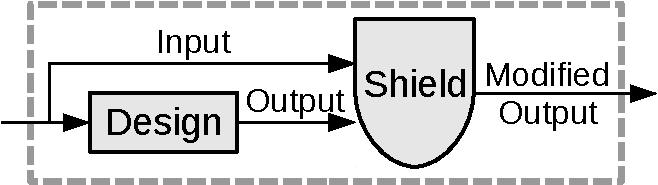
\includegraphics[width=0.75\textwidth]{MultiShield/figs/attach_shield}
\caption{Attaching a safety shield.}
\label{fig:attach_shield}
\vspace{-.3cm}
\end{figure}
\emph{Shield synthesis}~\cite{KonighoferABHKT17} is a general method to automatically derive runtime enforcement implementations, called shields,
from temporal logical specifications.
A shield is attached to a reactive system, monitors the behaviour of the system (i.e., its inputs and outputs), and corrects
erroneous outputs instantaneously, but only if necessary and as infrequently
as possible.


In this chapter, we introduce \emph{shield synthesis for multi-agent systems}. A shield monitors, and if needed corrects the output of one or more agents in the system, such that a given global safety specification is always satisfied. The distributed nature of the problem gives rise to a number of considerations to be made during the shield synthesis procedure. In order to explore the design space of possible shields for multi-agent systems, we categorize shields based on three criteria according to:
(1) the interference of the shield processes with the individual agents,
(2) the assumptions on the behaviour of the agents the shield can rely on, and
(3) the fairness of the shield w.r.t. the individual agents.


\emph{1.\ Quantifying interference.}
By construction, a shield is guaranteed to enforce correct operation of the shielded system. However, we might prefer one shield over another, based on how much the shield interferes with the system as a whole, or how it interferes with the individual agents in case of an error. In this chapter, we introduce the notion of  \emph{interference cost}
in order to quantify the quality of a shield
and synthesize cost-optimal shields that minimize the interference cost for the worst-case behavior of the multi-agent system.
We discuss different cost functions and provide algorithms to synthesize cost-optimal shields.

\emph{2.\ Assumptions on the multi-agent system.}
The shield synthesis procedure does not rely on the particular implementation of the system or specifications of each of the  agents, which is the key to the practicability of the approach. Instead, a shield has to guarantee safety for any possible implementation.
However, it is often realistic to make assumptions on the worst-case behavior of the system and  synthesize optimal shields w.r.t. the chosen interference cost under these assumptions. A natural assumption is that wrong outputs occur rarely, i.e., the length of all sequences of wrong outputs is bounded.
When such knowledge is available, we compute a cost-optimal shield considering the worst-case behavior of any system satisfying the assumptions.

\emph{3.\ Fair shielding.}
In the multi-agent setting, in which each individual agent might have to fulfill some individual goals, it is often important that a shield treats all agents fairly:
in case of an error, a fair shield does not always interfere with the same agent repeatedly.
In this chapter, we define a fairness notion for shields, and discuss the corresponding synthesis procedure.

\textbf{Contributions.}  We summarise our contributions as follows. To the best of our knowledge, this work is the first (1) to consider the automatic construction of runtime reinforcement modules
(we call them shields) for multi-agent systems, (2) to discuss synthesis of shields for multi-agent systems with quantitative objectives,
and (3) to construct shields under different assumptions on the behavior of the system.
We show the universality and potential of our approach on several examples.

